\newpage

\section{Experimenty}
\label{experiments}
V priebehu práce bolo nutné experimentovať v naozaj veľkom množstve s najrôznejším počtom vecí od typov neurónových sietí, datasetov až po rôzne prístupy k riešeniu zadaného problému.

Prvotné experimenty vykonávané vrámci predmetu Počítačové videnie\footnote{http://vgg.fiit.stuba.sk/teaching/computer-vision/} sú zachytené v kapitole \ref{first_experiments}. Ďalšie experimenty potom prebiehali postupne s konvolučnou neurónovou sieťou (kapitola \ref{experiments_cnn}), konvolučným autoenkóderom (kapitola \ref{experiments_autoencoder}) a autoenkóderom s predtrénovanou sieťou VGG-Net (kapitola \ref{experiments_vgg_net}). Pri každom modeli sme odskúšali nespočetné množstvo rôznych konfigurácií, pre popis sme ale vybrali len tie s najlepšími výsledkami pre jednotlivé časti. 

\subsection{Implementačné prostredie}

Všetky nižšie popisované experimenty boli naimplementované v jazyku Python za použitia najrôznejších knižníc, hlavne pre prácu s obrázkami a neurónovými sieťami. Najdôležitejšími knižnicami sú:
\begin{itemize}
	\item TensorFlow\footnote{https://www.tensorflow.org/} - open-source knižnica pre prácu s neurónovými sieťami a strojovým učením
	\item Keras\footnote{https://keras.io/} - vysoko úrovňová knižnica pre prácu s neurónovými sieťami, beží na nižšie úrovňovými knižnicami ako Theano či TensorFlow
	\item Matplotlib\footnote{https://matplotlib.org/} - knižnica pre 2D vykresľovanie v Python-e
	\item OpenCV\footnote{https://opencv.org/, https://pypi.org/project/opencv-python/} - open-source knižnica pre počítačové videnie a strojové učenie
	
	Trénovanie modelov v experimentoch prebiehalo na GPU.
\end{itemize}

\subsection{Prvotné experimenty}
\label{first_experiments}
Pre prvotné experimenty sme sa rozhodli zvoliť problém predikcie vizuálnej pozornosti v častiach obrázkov, konkrétne v tzv. regiónoch záujmu (z angl. regions of interest, ROIs), ktoré sme zvolili v okolí fixácií na obrázky.

\subsubsection{Úprava datasetu}
\label{dataset}

V tejto fáze prvotných experimentov sme pracovali s datasetom zloženým z niekoľkých voľne dostupných dataset-ov vizuálnej pozornosti (CAT2000\cite{borji2015cat2000}, NUSEF\footnote{http://mmas.comp.nus.edu.sg/NUSEF.html}, ...).
Keďže vo viacerých z nich chýbali úplné informácie k výpočtu máp výraznosti, rozhodli sme sa ich získať z dostupných obrázkov máp výraznosti, kedy sme ich načítali ako jednofarebný  obrázok v odtieňoch sivej (z angl. grayscale) - hodnota pixelu vtedy prakticky reprezentuje intenzitu. Ďalej sme spolu pre vstupné obrázky a mapy výraznosti extrahovali regióny záujmu, ktoré sme zvolili v okolí fixácií - vizualizácia popisovanej extrakcie je zobrazená na obrázku \ref{roi_image}. Nevyhovujúce časti datasetov (ako napr. abstraktné umienie, fraktály, cartoon obrázky, ...) boli odfiltrované.

\begin{figure}[H]
	\begin{center}
		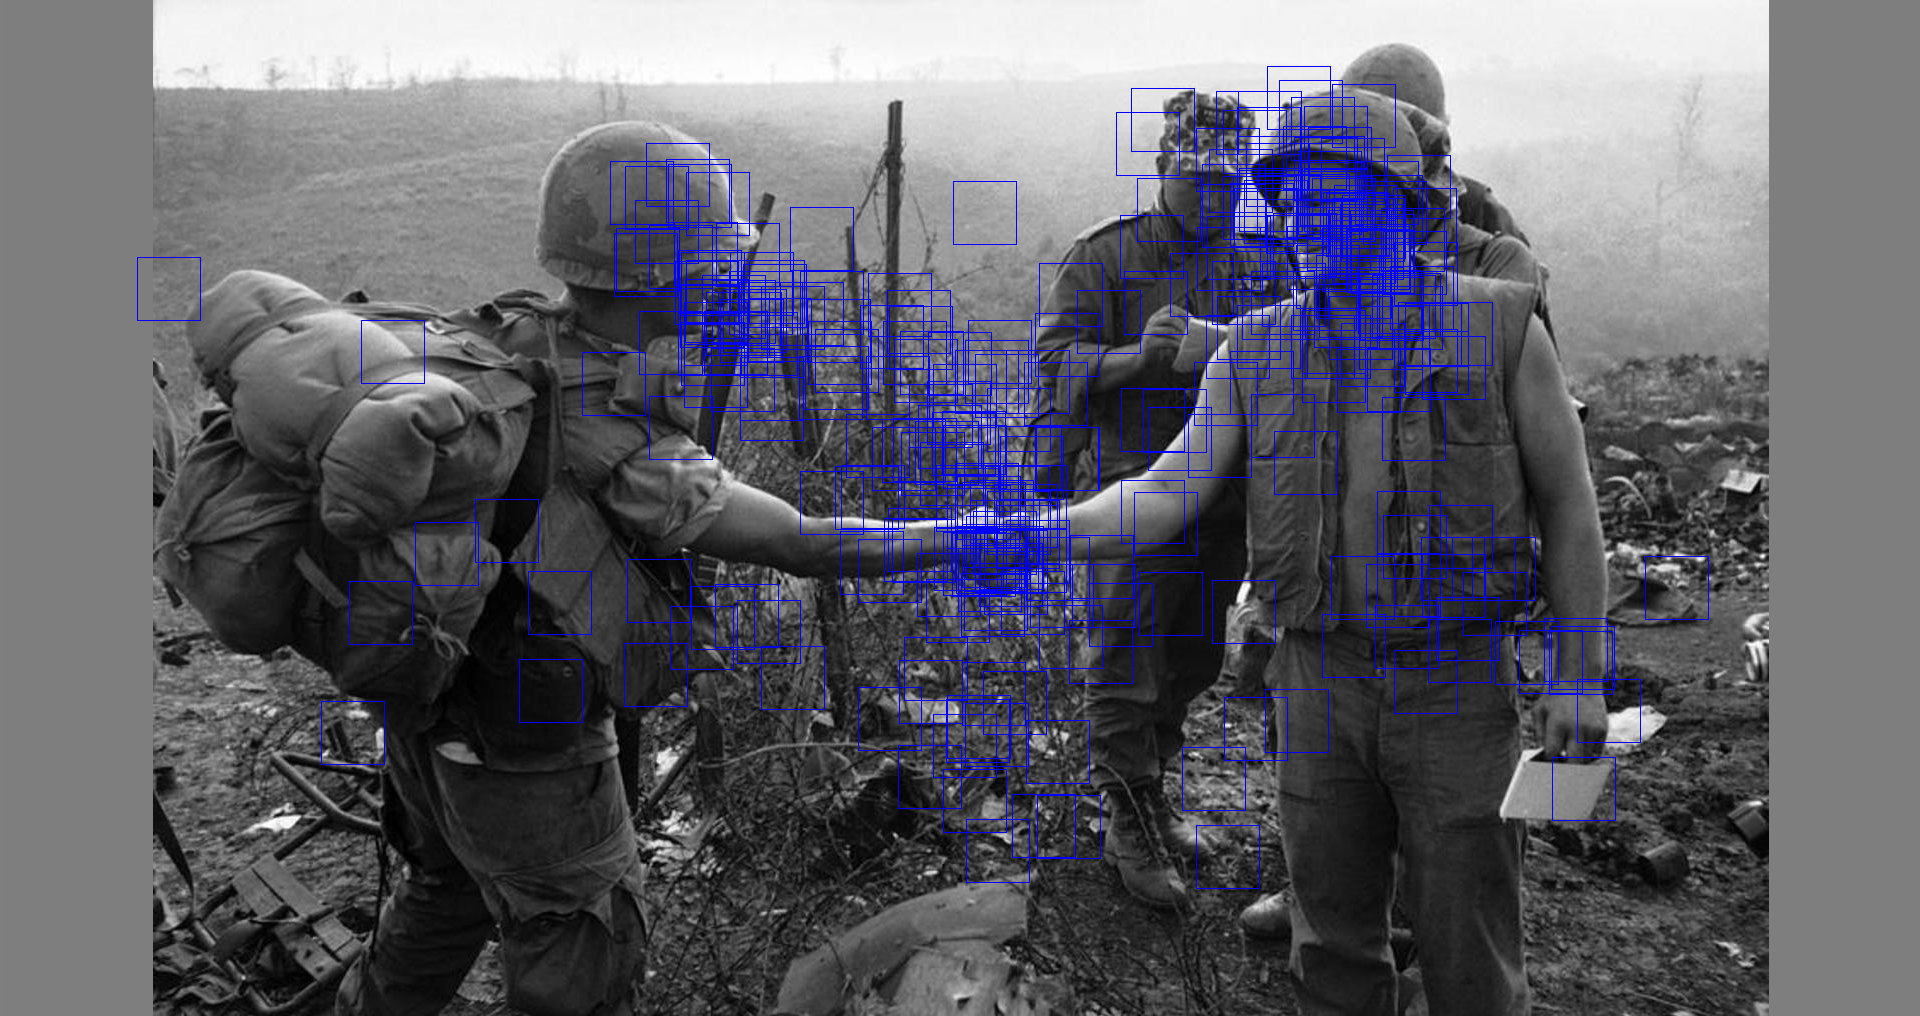
\includegraphics[scale=0.13]{img.PNG}
		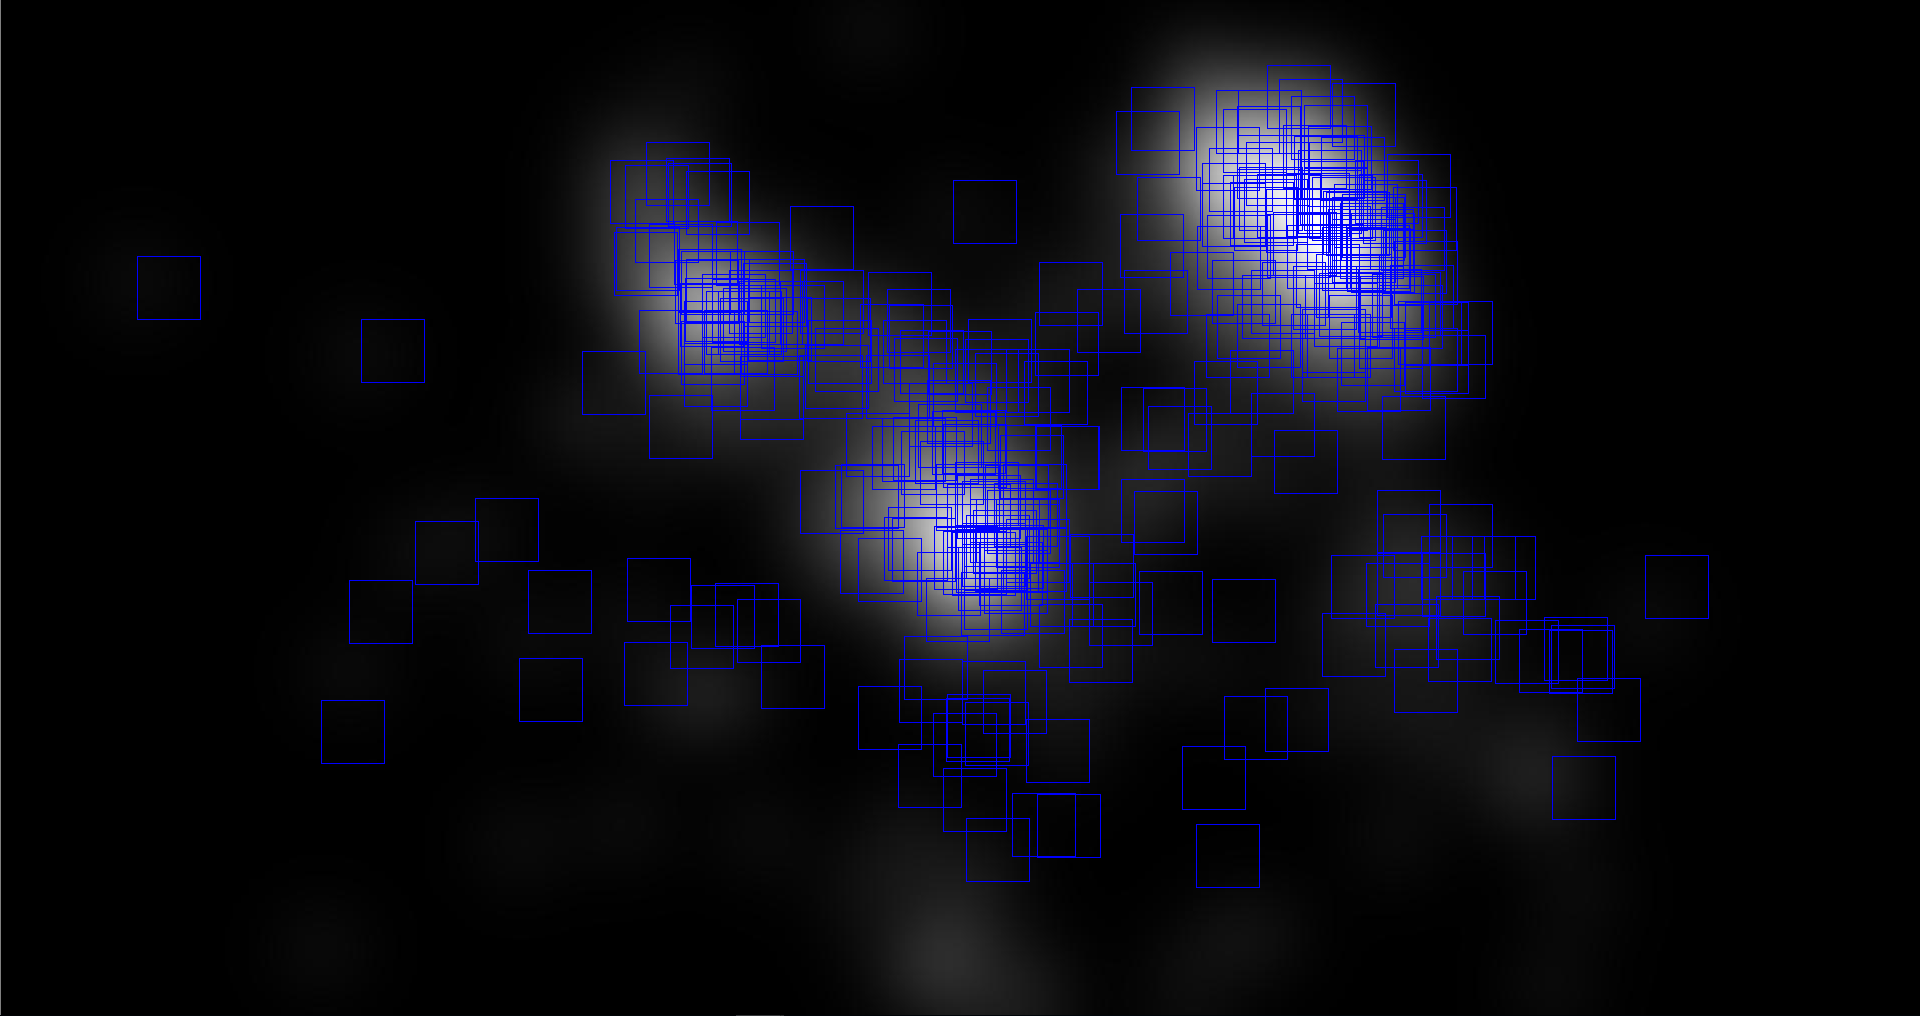
\includegraphics[scale=0.13]{map.PNG}
		\caption[Vizualizácia extrakcie regiónov záujmu]{
			Vizualizácia extrakcie regiónov záujmu, vľavo obrázok, vpravo mapa výraznosti k nemu
		}\label{roi_image}
	\end{center}
\end{figure}

Takto získané dáta boli ďalej pre neurónovú sieť normalizované, dokopy sme si nakoniec zaistili zhruba 500 000 vzoriek.
\newline

\subsubsection{Výsledky}

Navrhovanú konvolučnú neurónovú sieť (kapitola \ref{nn_popis}) sme trénovali na priravenom datasete, ktorý bol rozdelený štandardne v pomere 80:10:10 (80 - trénovanie, 10 - validácia, 10 - testovanie). Validácia prebiehala po každej iterácii a trénovanie končilo v momente keď sa chyba na validačných dátach začala výrazne odlišovať oproti najnižšej dosiahnutej (pomaly dochádzalo k pretrénovaniu). V závere mala sieť chybu predikcie na testovacích dátach na úrovni \textit{0.29}, chyba bola počítaná ako priemer chýb v každom bode obrázka. Na obrázku \ref{results_image} možno vidieť porovanie predikovaných máp výraznosti s originálnymi a so vstupnými obrázkami. 

\begin{figure}[H]
	\begin{center}
		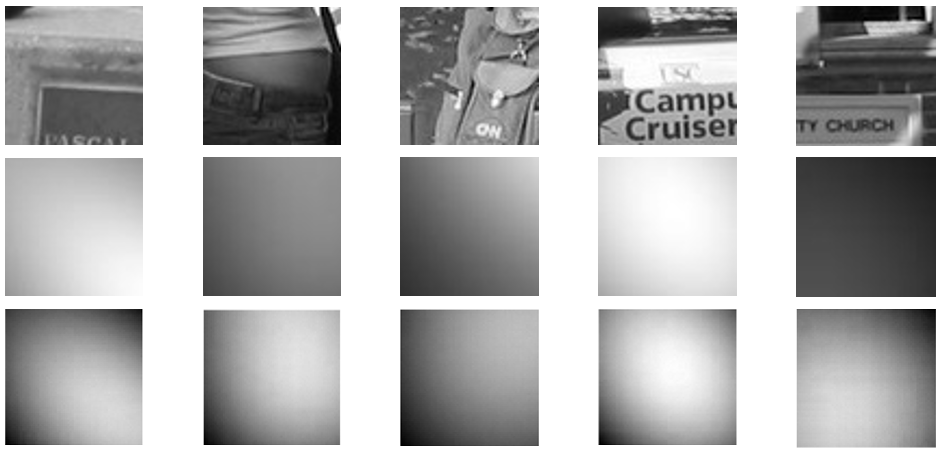
\includegraphics[scale=0.5]{predicted_saliency.PNG}
		\caption[Porovnanie prvotných výsledkov]{
			Porovnanie predikcií (dolu) s originálnymi mapami výraznosti (v strede) voči vstupným obrázkom (hore)
		}\label{results_image}
	\end{center}
\end{figure}

Pri snahe vypočítať metriky pre predikcie sme narazili na problém, ktorý sme si na začiatku neuvedomili. Väčšina metrík evaluuje mapu výraznosti voči binárnej matici reprezentujúcej fixácie na obrázok. Vzhľadom na to, že našim vstupom boli regióny záujmy v okolí fixácií, vo väčšine prípadov tieto binárne matice obsahovali len jednu fixáciu. Vďaka tomu mali metriky (AUC, sAUC, NSS) nezmyselne vysoké hodnoty. Z tohto dôvodu ich teda považujeme za nerelevantné a jediná metrika, podľa ktorej sa môžeme riadiť, je korelačný koeficient, keďže ten evaluuje predikovanú mapu voči tej pôvodnej. Jeho hodnoty na testovacích dátach sa v priemere pohybovali na hranici 0.563.

\subsection{Konvolučná neurónová sieť}
\label{experiments_cnn}

Ďalším experimentom bolo použitie klasickej konvolučnej neurónovej siete rovnako ako v predchádzajúcom prípade, tentokrát ale na celých obrázkoch. Ako dataset bol použitý spracovaný DUT-OMRON dataset (popísaný v kapitole \ref{dataset_description}) rozdelený podobne v pomere 80:10:10 (80 - trénovanie, 10 - validácia, 10 - testovanie), validácia bola tiež po každej epoche, trénovanie ale končilo v momente keď validačná chyba začala stúpať. Na obrázku nižšie možno vidieť vývoj jednotlivých chýb počas trénovania. Chyba bola počítaná ako priemier chýb predikcií v jednotlivých bodoch obrázka.

\begin{figure}[H]
	\begin{center}
	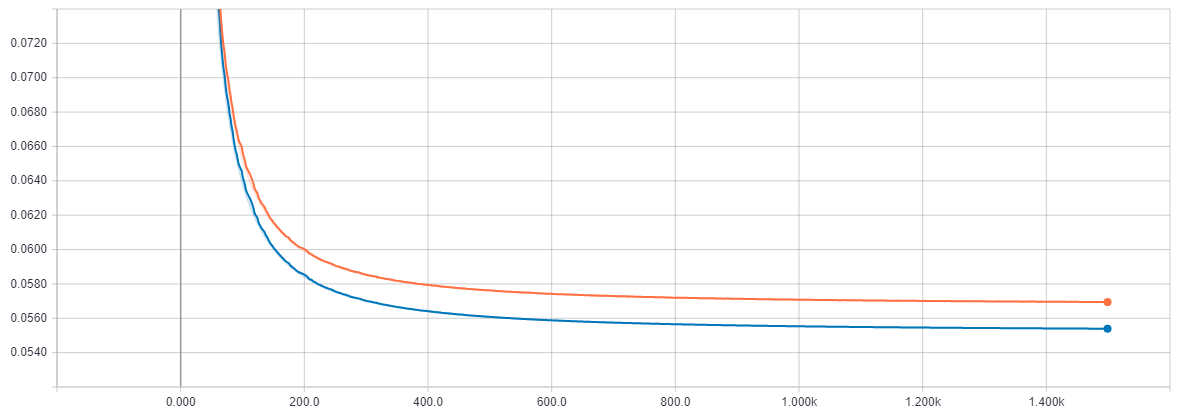
\includegraphics[scale=0.3]{nn_loss_no_outliers.png}
		\caption[Vývoj chyby počas trénovania konvolučnej neurónovej siete]{
			Graf zobrazujúci vývoj chyby neurónovej siete po odstránení extrémov počas 300 epoch - modrá farba reprezentuje chybu na trénovacích dátach, oranžová chybu na validačných dátach
		}\label{cnn_loss_outliers}
	\end{center}
\end{figure}

Z vyššie uvedených grafov vyplýva, že sieť bola schopná najvýraznejšie znížiť chybu predikcií behom prvých 50 epoch. Z jej počiatočnej hodnoty približne \textit{0.6709} klesla až na \textit{0.1321} na trénovacích dátach, na validačných dosahovala hodnotu \textit{0.1396}. Pri finálnom testovaní bola priemerná chyba približne \textit{0.1459}. Na prvý pohľad sa to môže javiť ako solídny výsledok, po vizualizovaní predikcií sme ale zistili, že sieť sa prakticky naučila predikovať ako najvýraznejšiu časť obrázka vždy len jeho stred, príklad predikcie je na obrázku \ref{cnn_results}.

\begin{figure}[H]
	\begin{center}
		
		%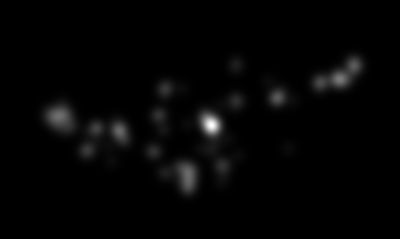
\includegraphics[width=10.58cm,height=6.32cm]{cnn_plane_heatmap.png}
		%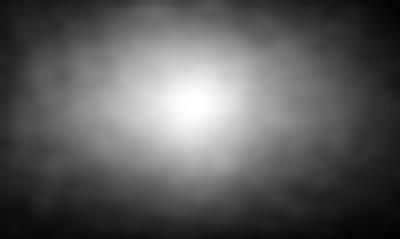
\includegraphics[width=10.58cm,height=6.32cm]{cnn_plane_predict.png}
		%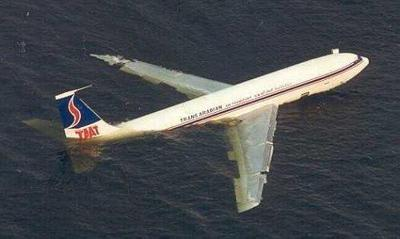
\includegraphics[width=10.58cm,height=6.32cm]{cnn_plane.png}
		%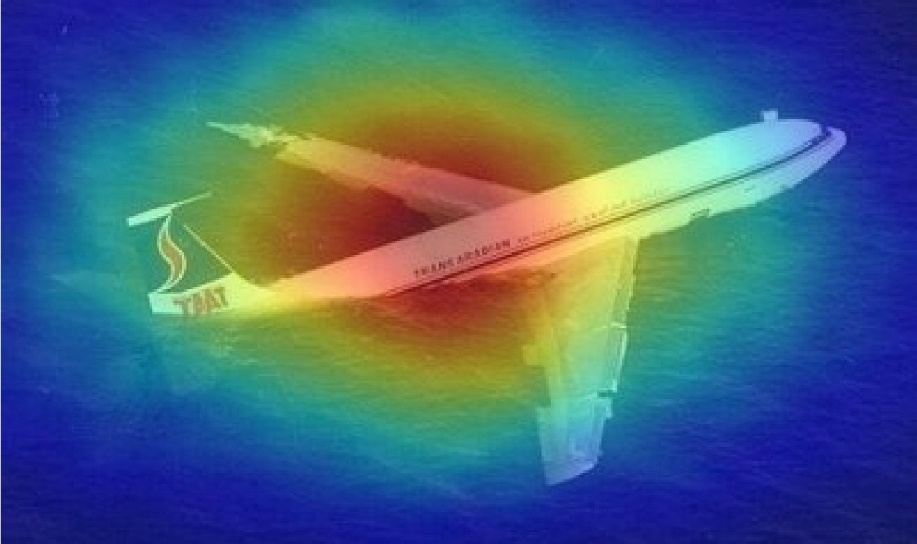
\includegraphics[width=10.58cm,height=6.32cm]{cnn_predict_on_plane.png}
		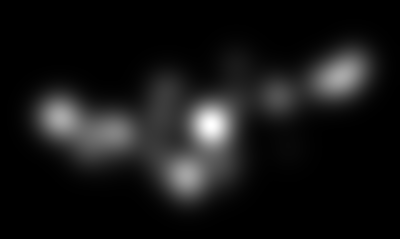
\includegraphics[scale=0.4]{cnn_plane_heatmap_regenerated.png}
		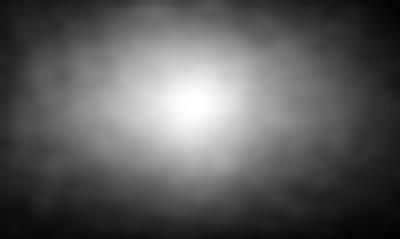
\includegraphics[scale=0.4]{cnn_plane_predict.png}
		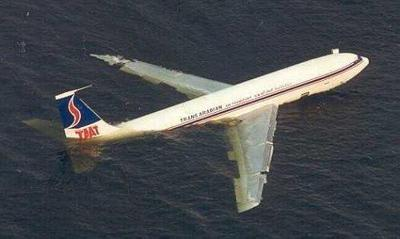
\includegraphics[scale=0.4]{cnn_plane.png}
		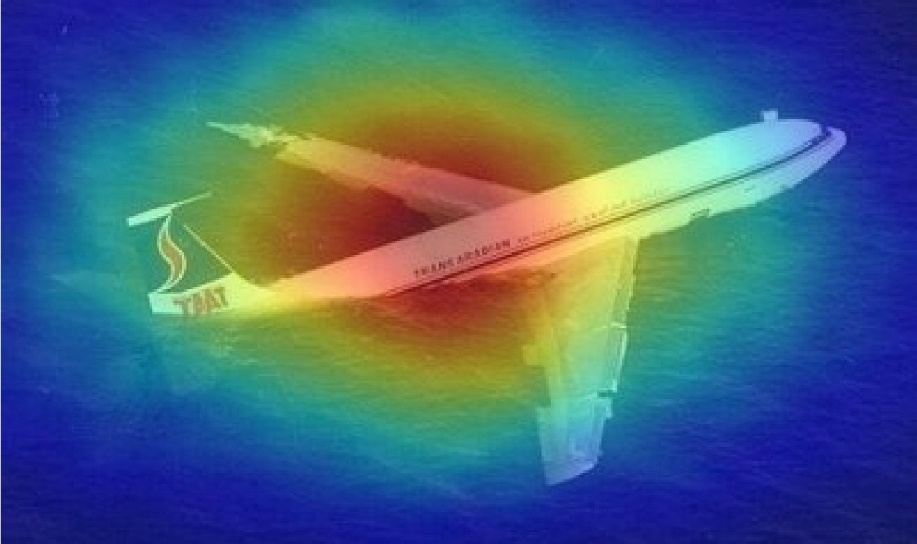
\includegraphics[scale=0.534]{cnn_predict_on_plane.png}
		\caption[Vzorka predikcie konvolučnej neurónovej siete]{
			Vľavo hore originálna mapa vizuálanej pozornosti, vpravo hore predikovaná mapa, vľavo dole obrázok pre prislúchajúce mapy výraznosti, vpravo dole zobrazenie predikcie na obrázku
		}\label{cnn_results}
	\end{center}
\end{figure}

Vyššie zobrazené správanie môže byť spôsobené napríklad relatívne malou veľkosťou vstupných obrázkov, kvôli veľkej pamäťovej náročnosti siete. 

\subsection{Konvolučný autoenkóder}
\label{experiments_autoencoder}

Ďalšou architektúrou, ktorú sme sa rozhodli vyskúšať, bol konvolučný autoenkóder (navrhnutý v kapitole \ref{autoencoder_design}. Použitý dataset a jeho rozdelenie bolo rovnaké ako v predošlom experimente, trénovanie ale končilo až keď validačná chyba za posledných \textit{n} epoch neklesla. Ako funkcia chyby bola použitá priemerná absolútna chyba (z angl. mean absolute error, MAE), ktorá meria rozdiel medzi dvomi spojitými premennými, v našom prípade medzi reálnou a predikovanou mapou výraznosti, resp. ich pixelmi. Priebeh učenia možno vidieť na obrázku \ref{autoencoder_loss}. 

\begin{figure}[H]
	\begin{center}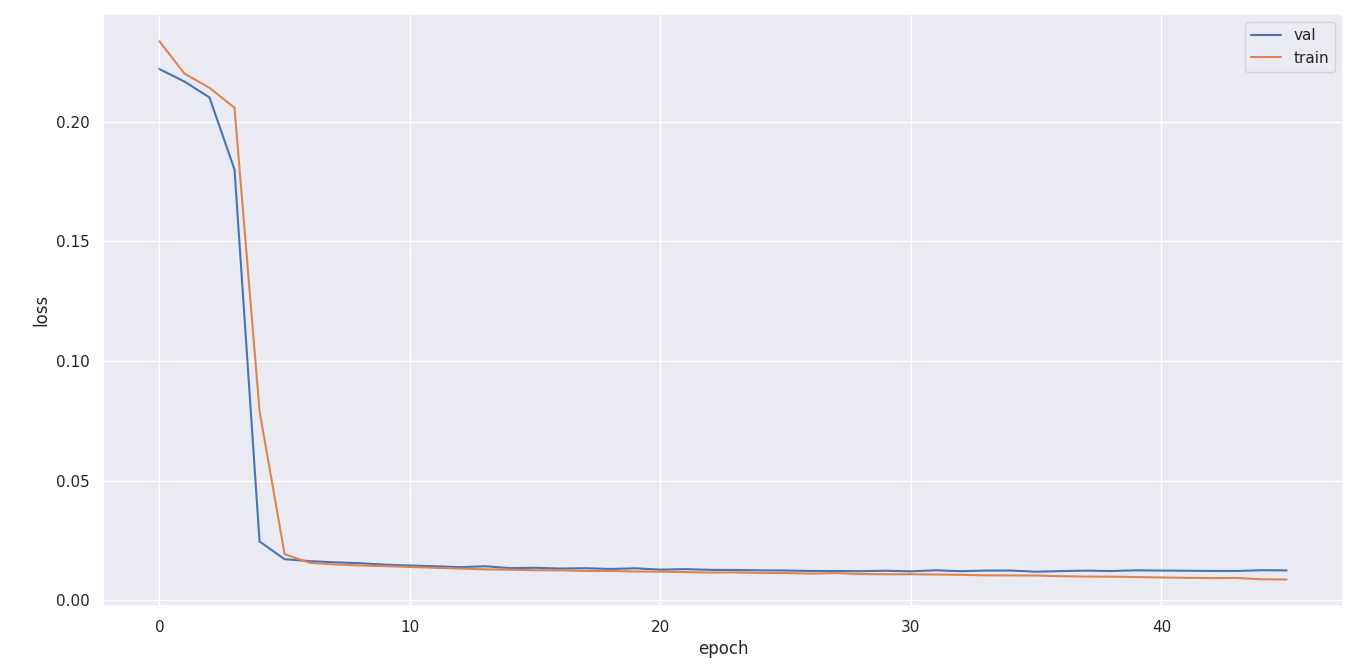
\includegraphics[scale=0.2]{autoencoder_loss.png}
		\caption[Vývoj chyby počas trénovania autoenkóderu]{
			Vývoj chyby počas trénovania, oranžovaná reprezentuje trénovaciu, modrá validačnú 
		}\label{autoencoder_loss}
	\end{center}
\end{figure}

Z obrázku je vidieť, že učenie prebiehalo počas 45 epoch, chyba najvýraznejšie klesla počas prvých šiestich epoch. Z počiatočnej hodnoty \textit{0.2336} (trénovacie dáta) a \textit{0.2219} (validačné dáta) bola schopná klesnúť až na hodnotu \textit{0.00874} (trénovacie dáta) a \textit{0.01245} (validačné dáta). Priemerná hodnota chyby pri testovaní na dátach, ktoré sieť nikdy nevidela, bola na úrovni \textit{0.01301}. Vizualizácie porovnanie predikcií sú zobrazené na obrázku \ref{autoencoder_results}.

\begin{figure}[H]
	\begin{center}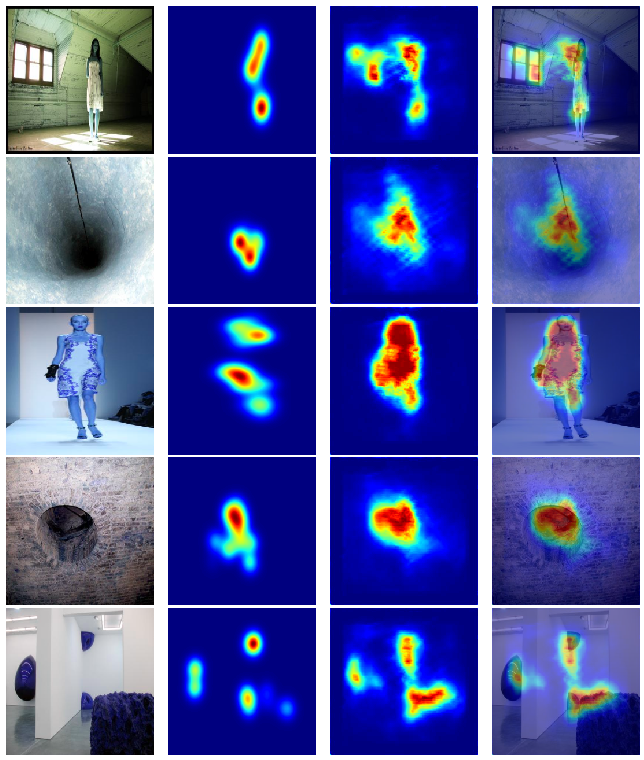
\includegraphics[scale=0.6]{autoencoder_results.png}
		\caption[Porovnanie predikcií autoenkóderu voči reálnym mapám výraznosti]{
			Porovnanie predikcií autoenkóderu, zľava vstupný obrázok, potom originálna mapa výraznosti, predikovaná mapa výraznosti a nakoniec predikcia zobrazená na obrázku. 
		}\label{autoencoder_results}
	\end{center}
\end{figure}

Z vyššie uvedených vizualizácií jasne vidieť, že sieť bola schopná naučiť sa isté výrazné súvislosti z dát, predikcie však nie sú úplne presné. Na rozdiel od siete z predošlého experimentu už nepredikuje všetko do stredu, ale je schopná označiť aj viacero výrazných objektov. To môže byť spôsobené napríklad väčšou veľkosťou vstupných obrázkov. Nakoľko autoenkóder si interne vstupné dáta zkomprimuje a zníži ich dimezionalitu, je v porovnaní zo spomínanou sieťou z predchádzajúceho experimentu pri rovnako veľkých vstupných obrázkoch menej pamäťovo náročný.

Zaujímavým javom, ktorý sme si všimli pri experimentovaní s týmto typom siete je, že hodnota chyby predikcie siete pri našom probléme nie je úplne smerodajná informácia. Pri použití napr. priemernej štvorcovej chyby (z angl. mean square error, MSE) bola výsledná chyba \textit{0.0000431}, ale predikcie boli v podstate len prázdne mapy bez akýchkoľvek výrazných častí. Tiež pri použití ešte väčšieho množstva konvlučných vrstiev sa použitá priemerná absolútna chyba zmenšila počas trénovania viac, avšak sieť sa v tomto prípade naučila predikovať najviac výrazné časti obrázkov vždy len do stredu, podobne ako pri konvolučnej neurónovej sieti z predošlého experimentu. Práve preto sme kvalitu modelov a predikcií vyhodnocovali metrikami vizuálnej pozornosti (kapitola \ref{metric}), ktorých prehľadné porovnanie aj so závermi je uvedené v \ref{results}.

\subsection{Autoenkóder s predtrénovaným modelom VGG-Net}
\label{experiments_vgg_net}

Pre tento experiment sme si vybrali sieť od A. Meyer-a\footnote{https://github.com/arthurmeyer/Saliency\_Detection\_Convolutional\_Autoencoder} popisovanú v kapitole \ref{object_detection}, ktorá je voľne dostupná. Jedná sa o variáciu autoenkóderu využívajúceho VGG-Net sieť k predikcii binárnej mapy zobrazujúcej dominantné objekty v scéne. Pôvodná hypotéza bola, že vďaka použitému predtrénovanému modelu VGG-Net pre detekciu objektov bude sieť lepšie rozumieť vstupný obrázkom a preto pri dodatočnom dotrénovaní k predikcii máp vizuálnej pozornosti bude dávať lepšie výsledky. Po menších úpravách siete sme pristúpili k trénovaniu na našom datasete, postupný vývoj chyby počas trénovania možno vidieť na obrázku \ref{vgg_pretrained_loss}. Validácia prebiehala každých 100 epoch, trénovanie končilo v momente keď minimálna hodnota chyby za posledných \textit{n} epoch neklesla. 
 
\begin{figure}[H]
	\begin{center}
		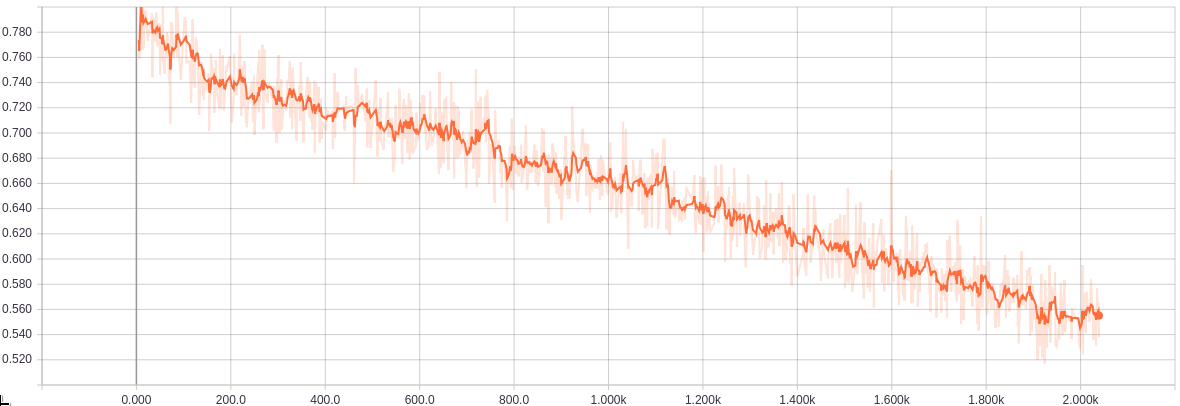
\includegraphics[scale=0.3]{vgg_pretrained.png}
		\caption[Vývoj chyby počas trénovanie siete s predtrénovaným modelom VGG-Net]{
			Graf zobrazujúci vývoj chyby po odstránení extrémov pri použití predtrénovaného modelu VGG-Net 
		}\label{vgg_pretrained_loss}
	\end{center}
\end{figure}

Na prvý pohľad sa môže zdať, že sieť sa bola schopná naučiť aspoň nejaké závislosti z dát. Po vizualizovaní dát sme ale zistili, že sme sa veľmi mýlili a snaha o dotrénovanie nepriniesla žiadne ovocie. Vizualizované výsledné dáta, ktoré mali reprezentovať mapy výraznosti, rozhodne ako mapy výraznosti nevyzerali a sieť sa nenaučila nič užitočné. Výsledkom boli len úplne náhodné hodnoty, ktoré sa ani zďaleko neblížili realite. Preto možno považovať tento experiment za nepríjemnú slepú uličku.

\subsection{Porovnanie výsledkov experimentov}
\label{results}
% TODO metriky sem nahodit 
\iffalse
cnn:

final correlation coeficient: 0.3891757367163311
final SIM: 0.30586936122666497
final NSS: 1.2774279939809017
final judd AUC: 0.8380535277085104
final shuffled AUC: 0.8247464580221275
final borji AUC: 0.8247464580221275


\fi
%multiline comment 
\iffalse
Počas zostrojovania neurónovej siete sme vykonali niekoľko experimentov, týkali sa hlavne konfigurácie siete, rôznych aktivačných funkcií, optimizérov a veľkosti datasetu pri trénovaní. Väčšie experimenty sú popísané v častiach \ref{val_vs_noval} a \ref{dropout_vs_nodropout}, zistenia z tých menších sú zhrnuté nasledovne:

\begin{itemize}
	\item najlepšie sa sieť učí, keď dostane naraz celý trénovací dataset, nie len jeho časti
	\item pridanie ďalších plne prepojených vrstiev predikcie zhoršilo
	\item pridanie viacerých konvolučných vrstiev nemalo prakticky žiadny vplyv na predikcie
	\item použitím štandardnej ReLU aktivačnej funkcie dosahovala chyba predikcie enormné hodnoty, bez ohľadu na rýchlosť učenia a použitý optimizér (Adam, Gradient descent, ...)
	\item aktivačná funkcia Sigmoid v kombinácii s Ftrl optimizérom, ktorého rýchlosť učenia bola 0.2, dávala najnižšiu chybu predikcií
\end{itemize}

Na základe vyššie uvedeného sme teda do ďalších experimentov pokračovali s modelom neurónovej siete, kde bola aktivačná funkcia Sigmoid, Ftrl optimizér, rýchlosť učenia 0.2 a rovnaký počet konvolučných a plne prepojených vrstiev ako v zobrazenom modeli v časti \ref{navrh}.

\subsection{Model s validáciou vs. model bez validácie}
\label{val_vs_noval}
Nakoľko máme dosť malý dataset, experimentovali sme s modelom, kde nebola použitá validácia a dáta pre ňu určené boli pridelené k trénovacím dátam. Výsledok však dosiahol iba zhoršenie priemernej chyby predikcie o 0.001. Tréning bez validácie končil v momente, keď chyba na tréningových dátach začala rásť, s validáciou končil až keď začala rásť na validačných dátach. To vyústilo vo viac ako 2x dlhší tréning, ako môžete vidieť na obrázku \ref{validation_graph}. 

	\begin{figure}[H]
			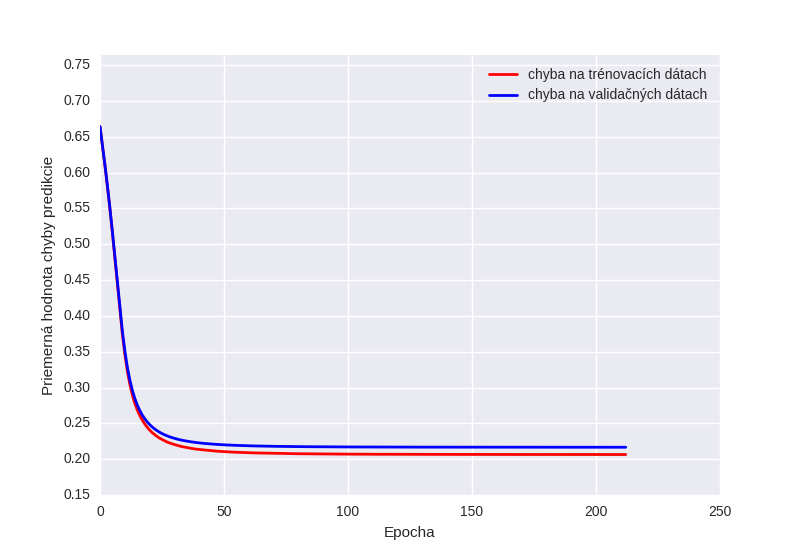
\includegraphics[scale=0.33]{train+val.png}
			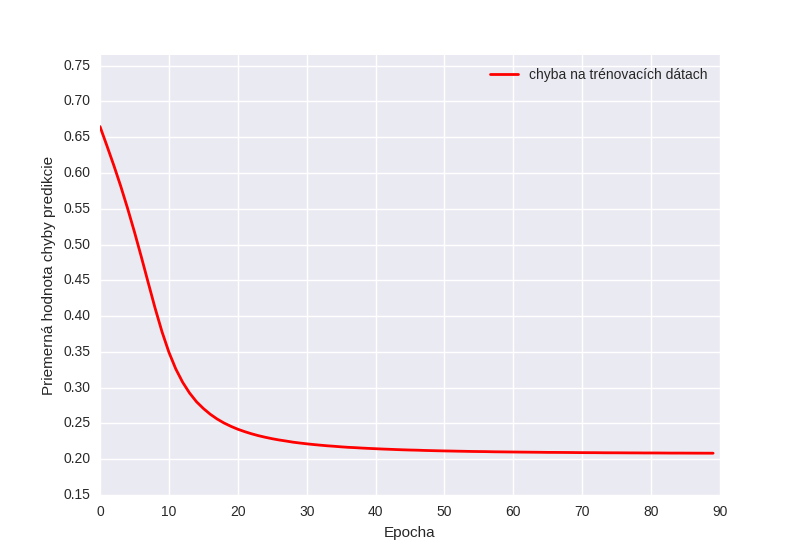
\includegraphics[scale=0.33]{train.png}
		\caption[Trénovanie s validáciou vs. trénovanie bez validácie]{Grafy poklesu chyby pri jednotlivých trénovaniach, vľavo trénovanie s validáciou, vpravo bez nej}\label{validation_graph}
	\end{figure}
	
Chyba na natrénovanom modeli bez validácia bola na testovacích dátach 0.2088, na trénovacích 0.2061. Na natrénovanom modeli s validáciou bola chyba na testovacích dátach 0.2078, na validačných 0.2166 a na trénovacích 0.2066. Takže zlepšenie bolo síce minimálne, ale stále badateľné. Hlavný dôvod, prečo validácia nemala až taký účinok, je malé množstvo dát. 

\subsection{Model s vrstvou výpadku vs. model bez vrstvy výpadku}
\label{model_graph}
\label{dropout_vs_nodropout}
Ďalšiu konfiguračnú zmenu, s ktorej implementáciou sme experimentovali, bolo pridanie vrstvy výpadku. Výsledok bol však len ten, že sieť sa dokázala naučiť to isté za rýchlejší čas, predikcie sa ale nezlepšili, ako je vidieť na nasledujúcich grafoch na obrázku \ref{dropout}. 

	\begin{figure}[H]
		
		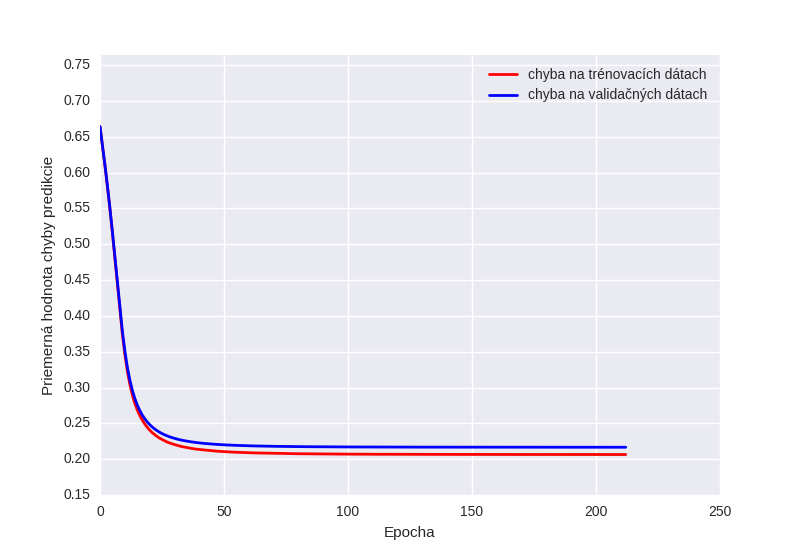
\includegraphics[scale=0.33]{train+val.png}
		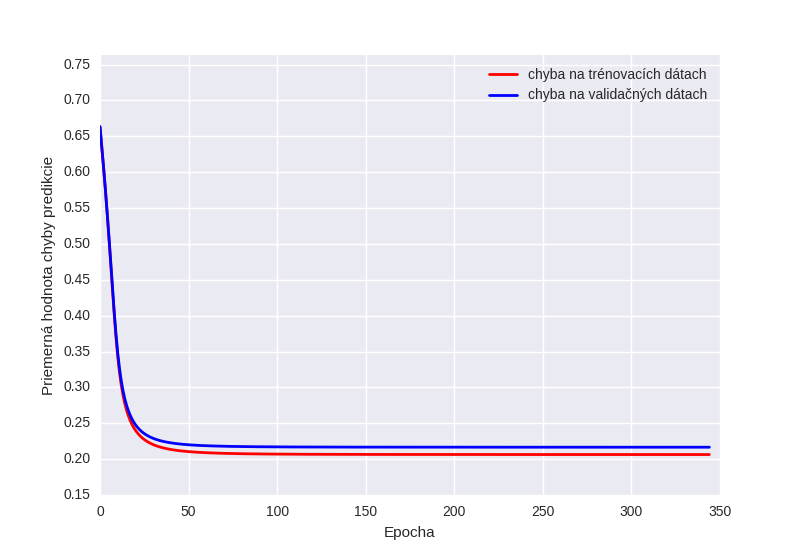
\includegraphics[scale=0.33]{without_dropout.png}
		\caption[Model s vrstvou výpadku vs. bez nej]{Grafy poklesu chyby pri jednotlivých trénovaniach, vľavo model s vrstvou výpadku, vpravo bez nej}\label{dropout}
	\end{figure}
	
\fi